\documentclass{article}
\usepackage[T1]{fontenc}
\usepackage{lmodern}
\usepackage{graphicx}
\usepackage{amsmath,amssymb}
\usepackage[a4paper,margin=2cm]{geometry}
\usepackage[absolute,overlay]{textpos}
\setlength{\TPHorizModule}{1mm}
\setlength{\TPVertModule}{1mm}
\usepackage[indonesian]{babel}
\usepackage{hyperref}
\setlength{\emergencystretch}{2em}
% unit: Halaman 23

\begin{document}

% === Halaman 23 (llm) ===

\vspace{212.65mm}

\section*{Deretan Kasus Dugaan Kebocoran Data di RI}

\vspace{80mm}

...dan masih banyak lagi

% deskripsi: Infografis timeline rangkaian kasus dugaan kebocoran data di Indonesia dari tahun 2020 hingga 2022, menampilkan bulan dan jumlah data yang bocor.
% bbox normalisasi: [0.1010, 0.1540, 0.5170, 0.8700]
\begin{textblock*}{87.36mm}(21.21mm,45.74mm)
\noindent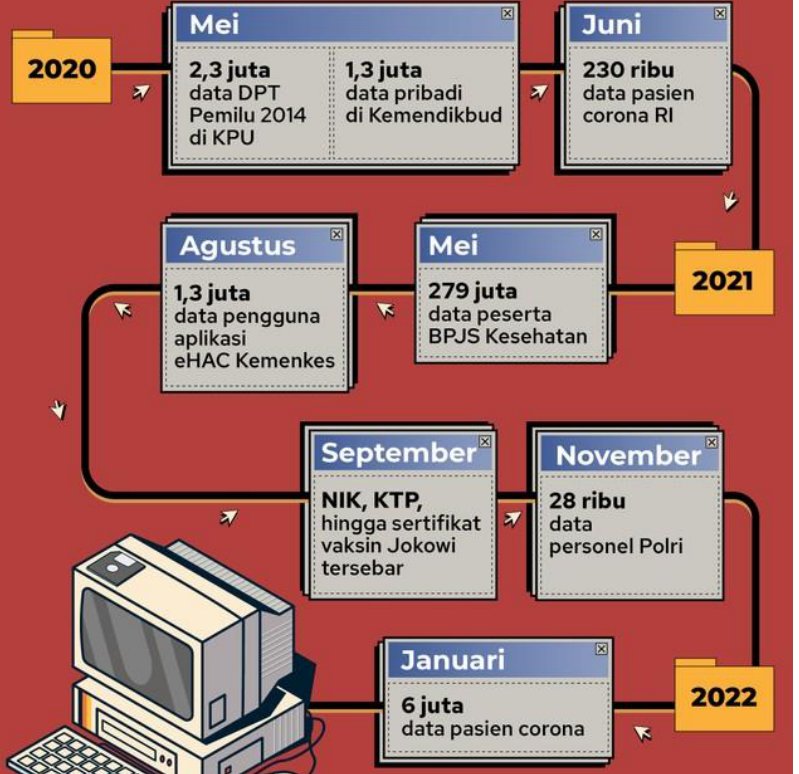
\includegraphics[width=87.36mm,height=212.65mm]{../../images/llm/page_023_img_01.png}%
\end{textblock*}

\end{document}
